%\documentclass[handout]{beamer}
%\documentclass[slidestop,compress,mathserif,12pt,t,professionalfonts,xcolor=table]{beamer}
\documentclass[]{beamer}
%\documentclass{beamer}
%\usepackage[dvips]{color}
\usepackage{graphicx}
\usepackage{amsmath,amssymb,array,comment,eucal}
\newcommand{\e}{\mathbf{e}}
\renewcommand{\P}{\mathbf{P}}
\newcommand{\F}{\mathbf{F}}
\newcommand{\R}{\textsf{R}}
\newcommand{\mat}[1] {\mathbf{#1}}
%\newcommand{\ind}{\mathrel{\mathop{\sim}\limits^{\mathit{ind}}}}
%\newcommand{\iid}{\mathrel{\mathop{\sim}\limits^{\mathit{iid}}}}
\newcommand{\E}{\textsf{E}}
\newcommand{\SE}{\textsf{SE}}
\newcommand{\SSE}{\textsf{SSE}}
\newcommand{\RSS}{\textsf{RSS}}
\newcommand{\FSS}{\textsf{FSS}}
\renewcommand{\SS}{\textsf{SS}}
\newcommand{\MSE}{\textsf{MSE}}
\newcommand{\SSR}{\textsf{SSR}}
\newcommand{\Be}{\textsf{Beta}}
\newcommand{\St}{\textsf{St}}
%\newcommand{\C}{\textsf{C}}
\newcommand{\GDP}{\textsf{GDP}}
\newcommand{\NcSt}{\textsf{NcSt}}
\newcommand{\Bin}{\textsf{Bin}}
\newcommand{\NB}{\textsf{NegBin}}
\renewcommand{\NG}{\textsf{NG}}
\newcommand{\N}{\textsf{N}}
\newcommand{\Ber}{\textsf{Ber}}
\newcommand{\Poi}{\text{Poi}}
\newcommand{\Gam}{\textsf{Gamma}}
\newcommand{\BB}{\textsf{BB}}
\newcommand{\Gm}{\textsf{G}}
\newcommand{\Un}{\textsf{Unif}}
\newcommand{\Ex}{\textsf{Exp}}
\newcommand{\DE}{\textsf{DE}}
\newcommand{\tr}{\textsf{tr}}
\newcommand{\cF}{{\cal{F}}}
\newcommand{\cL}{{\cal{L}}}
\newcommand{\cI}{{\cal{I}}}
\newcommand{\cB}{{\cal{B}}}
\newcommand{\cP}{{\cal{P}}}
\newcommand{\bbR}{\mathbb{R}}
\newcommand{\bbN}{\mathbb{N}}
\newcommand{\pperp}{\mathrel{{\rlap{$\,\perp$}\perp\,\,}}}
\newcommand{\OFP}{(\Omega,\cF, \P)}
\newcommand{\eps}{\boldsymbol{\epsilon}}
\newcommand{\1}{\mathbf{1}_n}
\newcommand{\gap}{\vspace{8mm}}
\newcommand{\ind}{\mathrel{\mathop{\sim}\limits^{\rm ind}}}
\newcommand{\simiid}{\ensuremath{\mathrel{\mathop{\sim}\limits^{\rm
iid}}}}
\newcommand{\eqindis}{\ensuremath{\mathrel{\mathop{=}\limits^{\rm D}}}}
\newcommand{\iid}{\textit{i.i.d.}}
\newcommand{\SSZ}{S_{zz}}
\newcommand{\SZW}{S_{zw}}
\newcommand{\Var}{\textsf{Var}}
\newcommand{\corr}{\textsf{corr}}
\newcommand{\diag}{\textsf{diag}}
\newcommand{\var}{\textsf{var}}
\newcommand{\Cov}{\textsf{Cov}}
\newcommand{\Sam}{{\cal S}}
\def\H{\mathbf{H}}
\newcommand{\I}{\mathbf{I}}
\newcommand{\Y}{\mathbf{Y}}
\newcommand{\tY}{\tilde{\mathbf{Y}}}
\newcommand{\Yhat}{\hat{\mathbf{Y}}}
\newcommand{\Yobs}{\mathbf{Y}_{{\cal S}}}
\newcommand{\barYobs}{\bar{Y}_{{\cal S}}}
\newcommand{\barYmiss}{\bar{Y}_{{\cal S}^c}}
\def\bv{\mathbf{b}}
\def\X{\mathbf{X}}
\def\tX{\tilde{\mathbf{X}}}
\def\x{\mathbf{x}}
\def\xbar{\bar{\mathbf{x}}}
\def\Xbar{\bar{\mathbf{X}}}
\def\Xg{\mathbf{X}_{\boldsymbol{\gamma}}}
\def\Ybar{\bar{\Y}}
\def\ybar{\bar{y}}
\def\y{\mathbf{y}}
\def\Yf{\mathbf{Y_f}}
\def\W{\mathbf{W}}
\def\L{\mathbf{L}}
\def\w{\mathbf{w}}
\def\U{\mathbf{U}}
\def\V{\mathbf{V}}
\def\Q{\mathbf{Q}}
\def\Z{\mathbf{Z}}
\def\z{\mathbf{z}}
\def\v{\mathbf{v}}
\def\u{\mathbf{u}}

\def\zero{\mathbf{0}}
\def\one{\mathbf{1}}
\newcommand{\taub}{\boldsymbol{\tau}}
\newcommand{\betav}{\boldsymbol{\beta}}
\newcommand{\alphav}{\boldsymbol{\alpha}}
\newcommand{\A}{\mathbf{A}}
\def\a{\mathbf{a}}
\def\K{\mathbf{K}}
\newcommand{\B}{\mathbf{B}}
\def\b{\boldsymbol{\beta}}
\def\bhat{\hat{\boldsymbol{\beta}}}
\def\btilde{\tilde{\boldsymbol{\beta}}}
\def\tb{\tilde{\boldsymbol{\beta}}}
\def\bg{\boldsymbol{\beta_\gamma}}
\def\bgnot{\boldsymbol{\beta_{(-\gamma)}}}
\def\mub{\boldsymbol{\mu}}
\def\tmub{\tilde{\boldsymbol{\mu}}}
\def\muhat{\hat{\boldsymbol{\mu}}}
\def\t{\boldsymbol{\theta}}
\def\tk{\boldsymbol{\theta}_k}
\def\tj{\boldsymbol{\theta}_j}
\def\Mk{\boldsymbol{{\cal M}}_k}
\def\M{\boldsymbol{{\cal M}}}
\def\Mj{\boldsymbol{{\cal M}}_j}
\def\Mi{\boldsymbol{{\cal M}}_i}
\def\Mg{{\boldsymbol{{\cal M}_\gamma}}}
\def\Mnull{\boldsymbol{{\cal M}}_{N}}
\def\gMPM{\boldsymbol{\gamma}_{\text{MPM}}}
\def\gHPM{\boldsymbol{\gamma}_{\text{HPM}}}
\def\Mfull{\boldsymbol{{\cal M}}_{F}}
\def\tg{\boldsymbol{\theta}_{\boldsymbol{\gamma}}}
\def\g{\boldsymbol{\gamma}}
\def\eg{\boldsymbol{\eta}_{\boldsymbol{\gamma}}}
\def\G{\mathbf{G}}
\def\cM{\cal M}
\def\D{\Delta}
\def \shat{{\hat{\sigma}}^2}
\def\uv{\mathbf{u}}
\def\l {\lambda}
\def\d{\delta}
\def\Sigmab{\boldsymbol{\Sigma}}
\def\Lambdab{\boldsymbol{\Lambda}}
\def\lambdab{\boldsymbol{\lambda}}
\def\Mg{{\cal M}_\gamma}
\def\S{{\cal{S}}}
\def\qg{p_{\boldsymbol{\gamma}}}
\def\pg{p_{\boldsymbol{\gamma}}}
\def\t{\boldsymbol{\theta}}  
\def\T{\boldsymbol{\Theta}}  
\usepackage{verbatim}
%\input{../lec_style.tex}
\usetheme{default}
\setbeamercolor{structure}{fg=cyan!90!black}
%\setbeamercolor*{palette primary}{use=structure,fg=white,bg=gray!60}
%\setbeamercolor*{palette quaternary}{fg=white,bg=cyan!30!black}

%\usecolortheme{orchid}
\title{Introduction to Linear Models}
\institute{Merlise Clyde}
\author{STA721 Linear Models Duke University \\
}
\date{August 25, 2015}
\logo{duke.eps}

\begin{document}
\maketitle
\section{Coordinates}
\begin{frame}
  \frametitle{Coordinates}
\begin{itemize}
\item Instructor: Merlise Clyde   \\ 214 Old Chemistry \\
 Office Hours MWF 1:00-2:0 or right after class (or by appointment)
\item Teaching Assistants:  Nicole Dalzell \& Shin Shirota

\item Course: Theory and Application of linear models from both a
frequentist (classical) and Bayesian perspective \pause
\item Prerequisites:   linear algebra and a mathematical statistics
  course covering likelihoods and distribution theory (normal, t, F,
  chi-square, gamma distributions) \pause
\item Introduce  R programming as needed \pause
\item Introduce  Bayesian methods, but assume that you are
  co-registered in 601 or have taken it previously \pause
\item more info on Course Website
  \url{http://stat.duke.edu/courses/Fall15/sta721}
\end{itemize}
  \end{frame}

\section{Course Overview}
\begin{frame}
  \frametitle{Introduction}
  Build ``regression'' models that relate a response variable to a
  collection of covariates  \pause
  \begin{itemize}
  \item Goals of Analysis?  \pause
    \begin{itemize}
    \item Predictive models 
    \item Causal interpretation
    \item Testing of hypotheses
    \item confirmatory  or validation analyses    
    \end{itemize}
 \item Observational versus Experimental data? \pause (Confounding) \pause
 \item Sampling Schemes \pause  Generalizibility \pause
 \item Statistical Theory \pause 
  \end{itemize}
\end{frame}

\begin{frame}
  \frametitle{Prostate Example}
 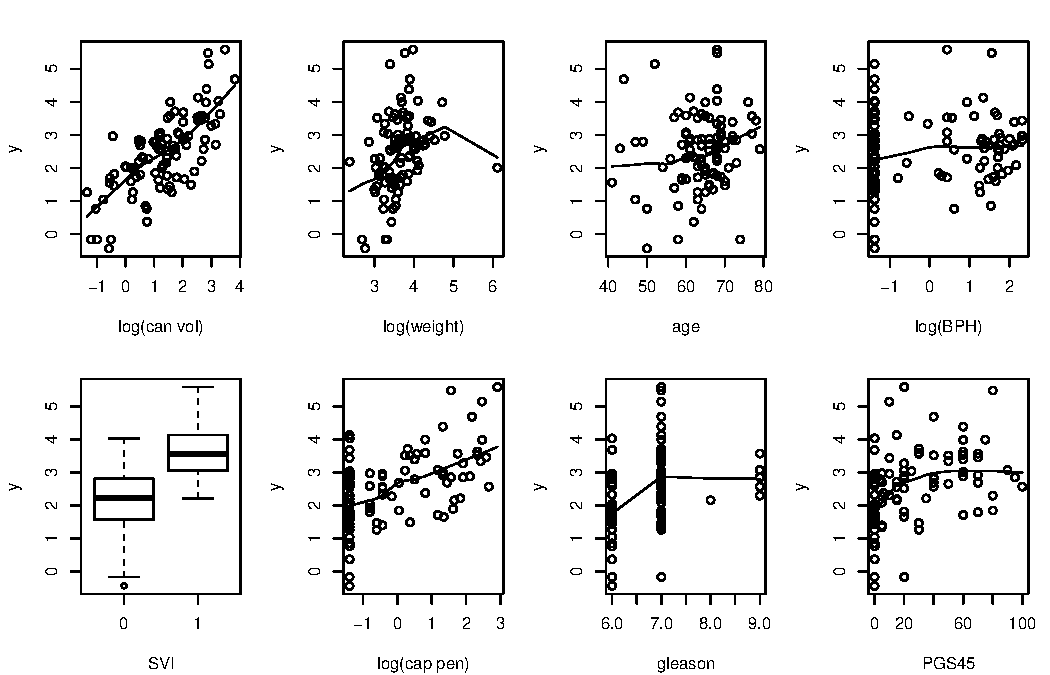
\includegraphics[height=3in]{prostfig1.pdf} 
\end{frame}
\begin{frame} \frametitle{Simple Linear Regression}
Simple Linear Regression:

$$y_i = \beta_0 + \beta_1 x_i + \epsilon_i \text{  for  } i = 1,
\ldots, n$$  \pause
 
Rewrite in vectors:

\begin{eqnarray*}
  \left[
\begin{array}{c}  y_1 \\ \vdots \\  y_n \end{array} 
  \right]   =  & 
 \left[ \begin{array}{c}  1 \\ \vdots \\ 1 \end{array}  \right]   \beta_0 + 
 \left[ \begin{array}{c}  x_1 \\ \vdots \\  x_n \end{array}
 \right] \beta_1 + 
\left[ \begin{array}{c}  \epsilon_1 \\ \vdots \\ \epsilon_n  \end{array}
\right]
\\
 & \\ \pause
\left[
\begin{array}{c}  y_1 \\ \vdots \\  y_n \end{array} 
  \right]   =  & 
 \left[ \begin{array}{cc}  1 &  x_1 \\ \vdots & \vdots \\ 1 & x_n\end{array}  \right]   
 \left[ \begin{array}{c}  \beta_0  \\  \beta_1 \end{array}
 \right] + 
\left[ \begin{array}{c}  \epsilon_1 \\ \vdots \\ \epsilon_n  \end{array}
\right] \\
 & \\ \pause
\Y = & \X \b + \eps
\end{eqnarray*}
\end{frame}

\begin{frame}
  \frametitle{Multiple Regression}
  $$y_i = \beta_0 + \beta_1 x_{1i} + \beta_2 x_{2i} + \ldots \beta_{p}
  x_{p i} + \epsilon_i$$

\pause
Design matrix  $$\X =
\begin{array}{cccc}
  1 & x_{11} & \ldots & x_{p1} \\
  1 & x_{12}  & \ldots & x_{p2} \\
  \vdots & \vdots  & \vdots & \vdots \\
  1 & x_{1n} & \ldots & x_{pn} \\
\end{array}
$$
\pause
$$\Y = \X \b + \epsilon$$
\pause
what should go into $\X$ and do we need all columns of $\X$ for
inference about $\Y$?
\end{frame}

\begin{frame}
  \frametitle{Nonlinear Models}
Mean function may be an intrinsically nonlinear function of $t$
  $$\E[Y_i] = f(t_i, \t)$$   

\centerline{ 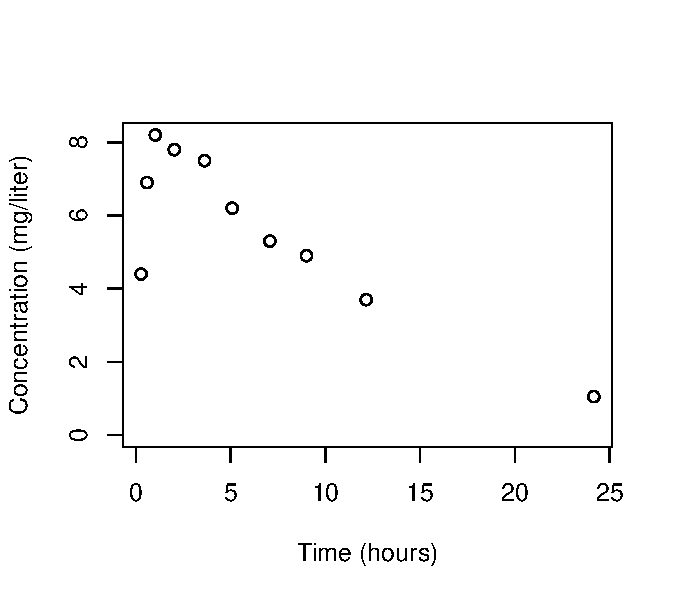
\includegraphics[height=2.5in]{theoph-fig1} }

\end{frame}
\begin{frame} \frametitle{Quadratic Linear Regression}
Taylor's Theorem:

$$f(t_i, \t) = f(t_0, \t) + (t_i - t_0) f'(t_0, \t) + (t_i - t_0)^2
\frac{f''(t_0, \t)}{2}  + R(t_i, \t)$$
\pause


$$y_i = \beta_0 + \beta_1 x_i + \beta_2 x_i^2 + \epsilon_i \text{  for  } i = 1, \ldots, n$$

\pause Rewrite in vectors:

\begin{eqnarray*}
\left[
\begin{array}{c}  y_1 \\ \vdots \\  y_n \end{array} 
  \right]   =  & 
 \left[ \begin{array}{ccc}  1 &  x_1 & x_1^2 \\ \vdots & \vdots \\ 1 &
     x_n &  x_n^2\end{array}  \right]   
 \left[ \begin{array}{c}  \beta_0  \\  \beta_1 \\ \beta_2 \end{array}
 \right] + 
\left[ \begin{array}{c}  \epsilon_1 \\ \vdots \\ \epsilon_n  \end{array}
\right] \\
 & \\ \pause
\Y = & \X \b + \eps \pause
\end{eqnarray*}

Quadratic in $x$, but linear in $\beta$'s, but remainder term is in
errors $\eps$
\end{frame}
\begin{frame} \frametitle{Polynomial Linear Regression}
Polynomial  Regression:

$$y_i = \sum_{j = 0}^q \beta_j x_i^j + \epsilon_i \text{  for  } i = 1, \ldots, n$$
\pause
Rewrite in vector  notation:

\begin{eqnarray*}
\left[
\begin{array}{c}  y_1 \\ \vdots \\  y_n \end{array} 
  \right]   =  & 
 \left[ \begin{array}{ccccc}  1 &  x_1 & x_1^2 & \ldots & x^q_1  \\
     \vdots & \vdots \\ 1 & x_n & x_n^2 & \ldots & x_n^q\end{array}  \right]   
 \left[ \begin{array}{c}  \beta_0  \\  \beta_1 \\ \beta_2 \\ \vdots \\ \beta_q \end{array}
 \right] + 
\left[ \begin{array}{c}  \epsilon_1 \\ \vdots \\ \epsilon_n  \end{array}
\right] \\
 & \\ \pause
\Y = & \X \b + \eps \pause
\end{eqnarray*}

How large should $q$ be?    \pause 

Use Nonlinear Regression  or other Nonparametric models

\end{frame}

\begin{frame} \frametitle{Kernel  Regression}
Kernel  Regression: 

$$y_i =  \beta_0 + \sum_{j = 1}^J \beta_j e^{-\lambda (x_i - k_j)^d} + \epsilon_i \text{  for  } i = 1, \ldots, n$$
where $k_j$ are kernel locations and $\lambda$ is a smoothing parameter
\pause
\begin{eqnarray*}
\left[
\begin{array}{c}  y_1 \\ \vdots \\  y_n \end{array} 
  \right]   =  & 
 \left[ \begin{array}{cccc}  1 &  e^{-\lambda (x_1 - k_1)^d} &
     \ldots &  e^{-\lambda (x_1 - k_J)^d}  \\
     \vdots & \vdots & & \vdots \\ 1 & e^{-\lambda (x_n - k_1)^d} &  \ldots & e^{-\lambda (x_n - k_J)^d} \end{array}  \right]   
 \left[ \begin{array}{c}  \beta_0  \\  \beta_1 \\\vdots \\ \beta_J \end{array}
 \right] + 
\left[ \begin{array}{c}  \epsilon_1 \\ \vdots \\ \epsilon_n  \end{array}
\right] \\
 & \\ 
\Y = & \X \b + \eps
\end{eqnarray*} \pause
Linear in $\beta$ given $\lambda$ \\  \pause
 
Learn $\lambda$  and $J$


\end{frame}

\begin{frame}
  \frametitle{Kernel Regression Example}
  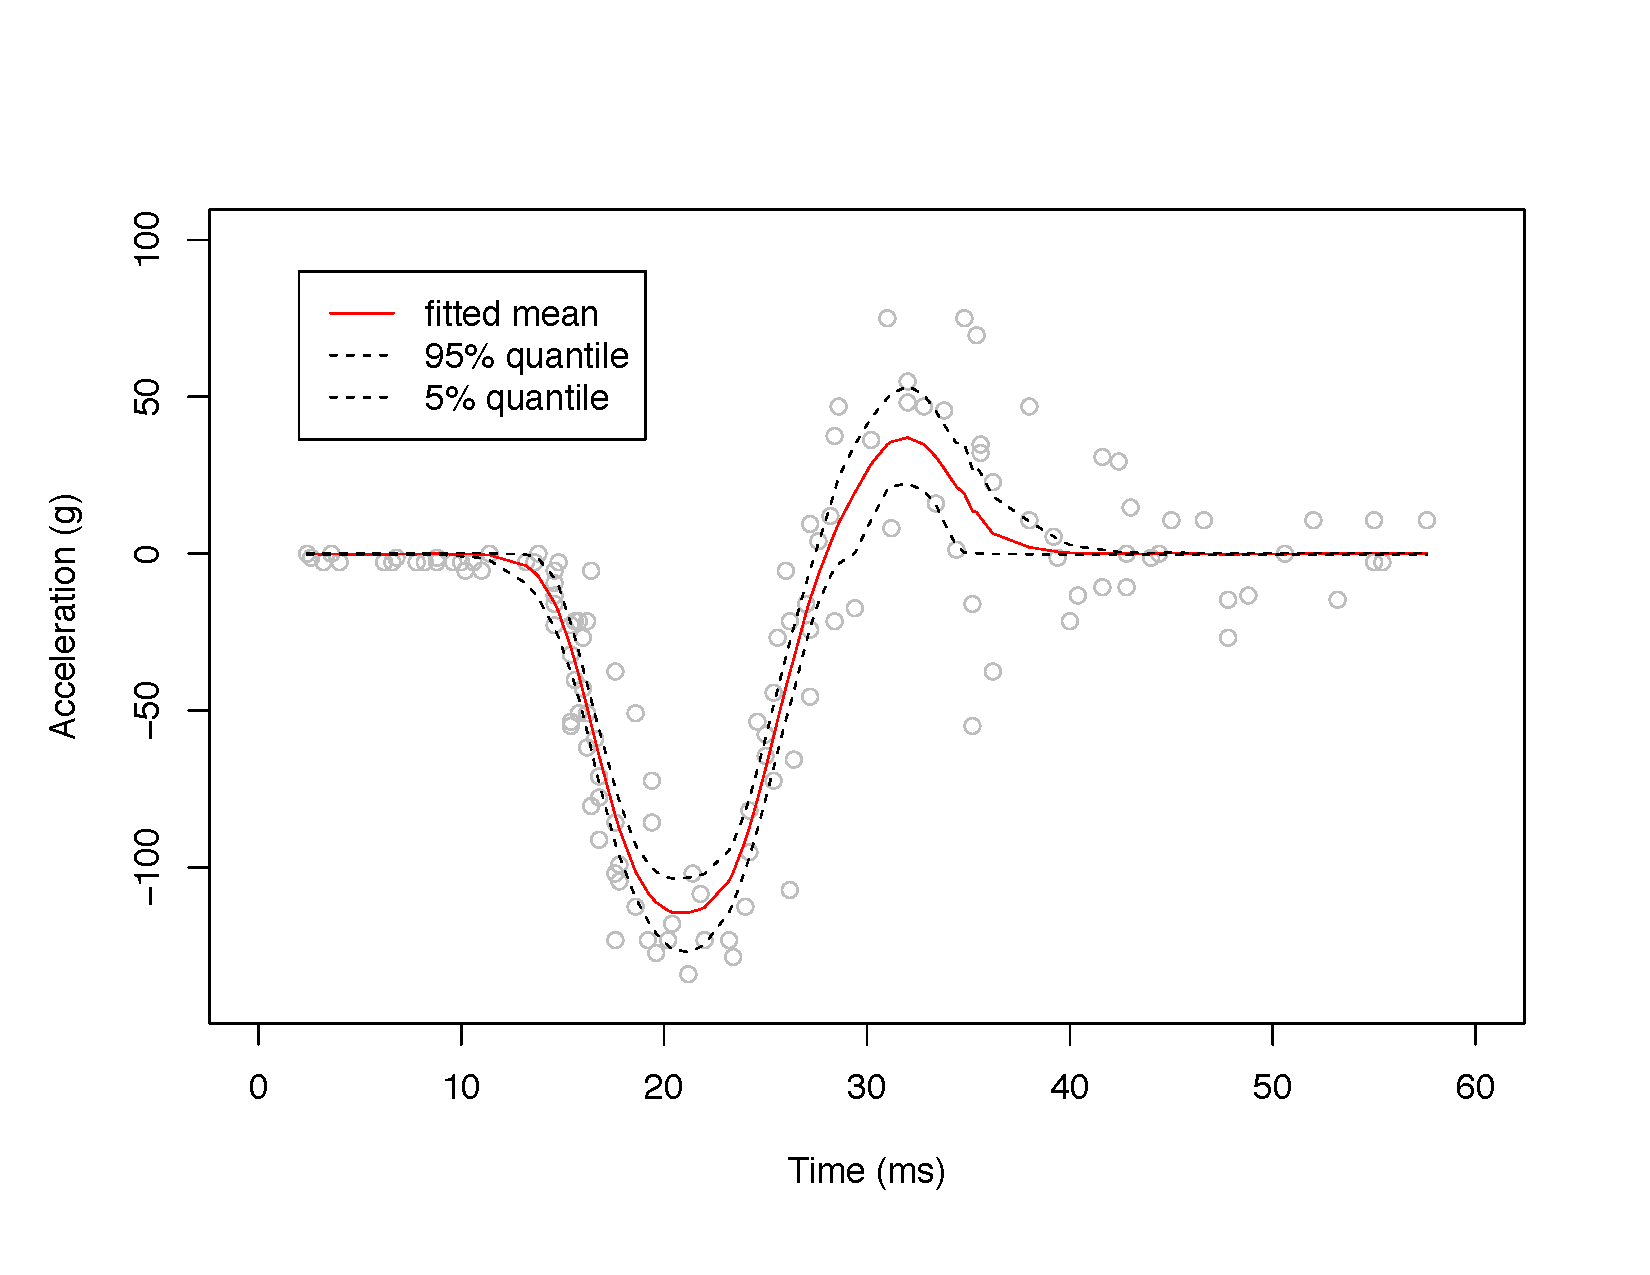
\includegraphics[height=3in]{/Users/mclyde/Documents/sta244/Lectures/Intro/motorcycle.pdf}
\end{frame}
\begin{frame}
  \frametitle{Hierarchical Models - Spinal Bone Density}
\centerline{  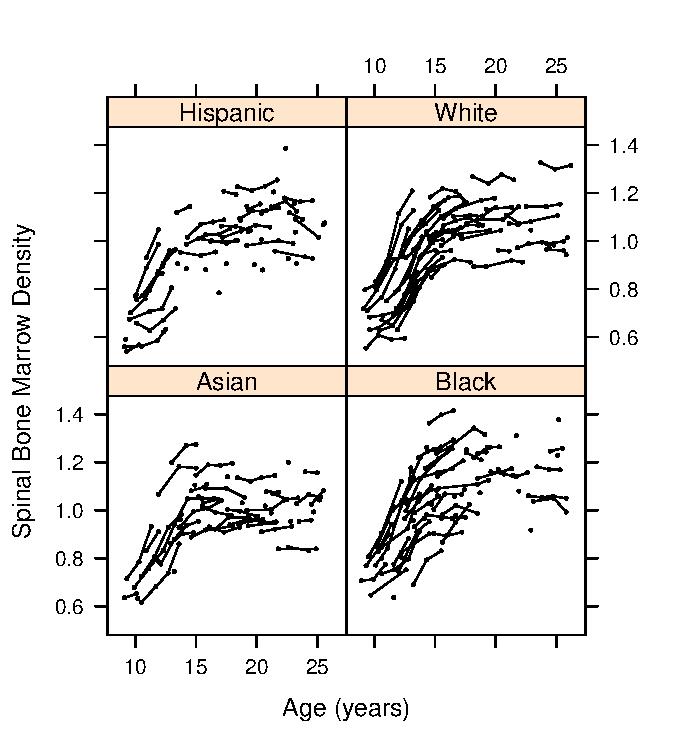
\includegraphics[height=3.5in]{spinalbone}}
\end{frame}

\begin{frame}
  \frametitle{Generic Linear  Model}
  Generic Model in Matrix Notation is
$$
\Y  = \X \, \b + \eps  $$
\pause
\begin{itemize}
\item $\Y$ ($n \times 1$) vector of response   (observe)
\item $X$ ($n \times p$)  design matrix  (observe)
\item $\b$ ($p \times 1$) vector of coefficients  (unknown)
\item $\eps$ ($n \times 1$) vector of ``errors''  (unobservable)
\end{itemize} \pause

Goals: \pause
\begin{itemize}
\item What goes into $\X$?   (model building and model selection) \pause
\item What if several models are equally good?  (model averaging) \pause
\item What about the future?  (Prediction) \pause
\item uncertainty quantification - assumptions about $\eps$\pause
\end{itemize}
{\it All models are wrong, but some may be useful }  (George Box)
\end{frame}

\begin{frame}
  \frametitle{Ordinary Least Squares}
  Goal: Find the best fitting ``line'' or ``hyper-plane'' that
  minimizes
$$\sum_i  (Y_i - \x_i^T \b)^2 = (\Y - \X\b)^T(\Y - \X \b) = \| \Y -
\X\b \|^2 $$  \pause

\begin{itemize}
\item Optimization problem \pause
\item May over-fit $\Rightarrow$ add other criteria that provide a penalty
  ``Penalized Least Squares'' \pause
\item Robustness to extreme points $\Rightarrow$ replace quadratic
  loss with other functions  \pause
\item no notion of uncertainty of estimates  \pause
\item no structure of problem  (repeated measures on individual,
  randomization restrictions, etc)
\end{itemize}
Need  Distribution Assumptions of $Y$ (or $\eps$) for testing and
uncertainty measures \pause $\Rightarrow$ Likelihood  and Bayesian inference
\end{frame}

\begin{frame}
  \frametitle{Philosophy}
  \begin{itemize}
\item for many problems frequentist and Bayesian methods will give
  similar answers (more a matter of taste in interpretation)
  \item For small problems, Bayesian methods allow us to incorporate
    prior information which provides better calibrated answers
  \item for problems with complex designs and/or missing data Bayesian
    methods are often easier to implement (do not need to rely
    on asymptotics)
\item For problems involving hypothesis testing or model selection
  frequentist and Bayesian methods can be strikingly different.
\item Frequentist methods often faster (particularly with ``big
  data'') so great for exploratory analysis and for building a
  ``data-sense''
\item Bayesian methods sit on top of Frequentist Likelihood
  \end{itemize}
Important to understand advantages and problems of each perspective!
\end{frame}
\end{document}
\section{Random Vectors}
\begin{frame}
  \frametitle{Random Vectors}
  Let $Y_1, \ldots Y_n$ be random variables in $\bbR$ \\ \pause
 Then $\Y \equiv
\left[ \begin{array}{c}
  Y_1 \\ 
\vdots \\
Y_n
\end{array} \right]$ is a random vector in $\bbR^n$ 


 

\end{frame}

\begin{frame}
  \frametitle{Expectations}
Mean or expected value $\E[Y_i] = \mu_i$   \\

Expectations of random vectors are defined element-wise:


$$\E[\Y] \equiv
\E \left[ \begin{array}{c}
  Y_1 \\ 
\vdots \\
Y_n
\end{array} \right] \equiv 
\left[ \begin{array}{c}
  \E[Y_1] \\ 
\vdots \\
\E[Y_n]
\end{array} \right] =
\left[ \begin{array}{c}
  \mu_1 \\ 
\vdots \\
\mu_n
\end{array} \right]
\equiv \mub \in \bbR^n
$$


\end{frame}

\begin{frame}
  \frametitle{Random Matrix}
  Likewise $\W = [w_{ij}]$ is a matrix $(r \times s)$ with elements
  $w_{ij}$ random variables in $\bbR$ \pause

Then $\E[\W] = [ \E[w_{ij}] ]$ defined element-wise \pause

 \begin{itemize} 
 
  \item $\Var[Y_i] = \sigma_i$ (variance) \pause 
 \item $\Cov(Y_i, Y_j) = \sigma_{ij}$ (covariance) \pause
  \end{itemize}

\begin{definition}
  $$\Cov(\Y) = \E[(\Y - \mub)(\Y - \mub)^T] =
 \left[ \begin{array}{ccc}
    \sigma_1 &  \ldots &\sigma_{1n} \\
    \vdots &  \sigma_2 \ldots \\
    \vdots & \ddots & \vdots \\
    \sigma_{n1} & \ldots & \sigma_n 
  \end{array} \right] \equiv \Sigma
$$
\end{definition}
\end{frame}
\begin{frame}
  \frametitle{Details}
  $\Cov(\Y) = \E[(\Y - \mub)(\Y - \mub)^T]$
\end{frame}

\begin{frame}
  \frametitle{Linear Transformations}
  If $\Y$ $(n \times 1)$ is a random variable and $\A$ is a $r \times
  n$ matrix and $\bv \in \bbR^n$ \pause

  then
$$\E[\A \Y + \bv] = \A \E[\Y] + \bv
$$
and \pause
$$\Cov[\A \Y + \bv] = \A \Cov[\Y] \A^T $$

This last result can be used to show that for an random variable $\Y$
$\Cov(\Y) \ge 0$  (non-negative definite) \pause


\end{frame}
\begin{frame}
  \frametitle{Positive and Non-Negative Definite}
  \begin{definition}
    A matrix $\Sigma$ $(n \times n)$ is positive definite ($\Sigma >
    0$) if for any
    non-zero $\v \in \bbR^n$ $\v^T \Sigma \v > 0$.   If $\v^T\Sigma \v
    \ge 0$ then $\Sigma$ is non-negative definite, $\Sigma \ge 0$
  \end{definition} \pause

We say that $\Y$ is non-singular if and only if $\Cov(\Y) > 0$
\end{frame}
\begin{frame}
  \frametitle{Distribution Theory}
  Need to define Multivariate Normal  (Read Section 1.2 and Appendix
  D, as well as review Appendix A \& B)
\end{frame}
\end{document}


\begin{frame} \frametitle{Linear Models}

  For a $d$ dimensional multivariate normal random vector, we write $\Y \sim N_d(\mub, \Sigmab)$
\pause
  \begin{itemize}
  \item<2-> $\E[\Y] = \mub$:  $d$ dimensional vector with means $E[Y_j]$
  \item<3-> $\Cov[\Y] = \Sigmab$: $d \times d$ matrix with diagonal elements
    that are the variances of $Y_j$ and off diagonal elements that are
    the covariances $\E[(Y_j - \mu_j)(Y_k - \mu_k)]$
  \end{itemize}
 \only<4>{ \begin{block}{Density}
 If $\Sigmab$ is positive definite ($\x'\Sigmab \x > 0$ for any $\x \ne
  0$ in $\bbR^d$) then $\Y$ has  a density with respect to Lebesgue
  measure on $\bbR^d$

$$p(\Y) = (2 \pi)^{-d/2} |\Sigmab|^{-1/2} \exp(-\frac{1}{2}(\Y - \mub)^T
\Sigmab^{-1} (\Y - \mub))$$    
  \end{block}}
\end{frame}
\frame{ \frametitle{Multivariate Normal Density}
\begin{itemize}
 \item<1-> Density of $Z \sim \N(\zero, \I_d)$:
\begin{eqnarray*}
\onslide<2->{f_{\Z}(\z) & = \prod_{j=1}^d \frac{1}{ \sqrt{2 \pi}} e^{-z_i^2/2} } \\
\onslide<3->{ \, & = (2\pi)^{-d/2}e^{- \frac{1}{2} (\Z^T\Z)}}
\end{eqnarray*}
\item<4-> $\Y = \mub + \A \Z$  
\item<5-> Solve for $\Z = g(\Y)$ 
\item<6-> Jacobian of the
  transformation  $J(\Z \rightarrow \Y) = | \frac{\partial
    g}{\partial \Y} |$ 
\item<7>substitute  $g(\Y)$ for $\Z$ in density and
  multiply by Jacobian
{$$  f_\Y(\y)  = f_\Z(\z) J(\Z \rightarrow \Y) $$}
\end{itemize}
}
\frame{ \frametitle{Multivariate Normal Density}
   \begin{equation} \Y  \eqindis \mub + \A \Z   \quad    \text{ for }  \Z \sim \N(\zero, \I_d) \end{equation}

  \begin{proof}
  \begin{itemize}
   \item<2->  since  $\Sigmab > 0, \, \exists$
   an $\A$ ($d \times d$) such that $\A > 0$ and $\A
  \A^T = \Sigmab$ 
\item<3-> { $\A >0  \Rightarrow   \A^{-1}$ exists}
\item<4-> Multiply both sides (1)  by $\A^{-1}$: $$\alert<4>{\A^{-1}}\Y =
  \alert<4>{\A^{-1}} \mub + \alert<4>{\A^{-1}}\A \Z$$
\item<5-> Rearrange $\A^{-1} (\Y - \mub) = \Z $ 
\item<6-> Jacobian of transformation $d\Z = |\A^{-1}| d\Y$
\item<7->  Substitute and simplify  algebra
  \end{itemize}
\onslide<7>{$$f(\Y) = (2 \pi)^{-d/2} |\Sigmab|^{-1/2} \exp(-\frac{1}{2}(\Y - \mub)^T
\Sigmab^{-1} (\Y - \mub))$$  }
  \end{proof}
  
}

\frame{ \frametitle{Zero Correlation and Independence}
 \begin{theorem}
For a random vector $\Y \sim \N(\mub, \Sigmab) $ partitioned as
$$
\Y = \left[
  \begin{array}{c}
\Y_1  \\ \Y_2 \end{array} \right]  \sim \N\left( \left[
  \begin{array}{c} \mub_1  \\ \mub_2 \end{array} \right],
  \left[ \begin{array}{cc}
\Sigmab_{11} &  \Sigmab_{12}  \\ 
\Sigmab_{21} & \Sigmab_{22} \end{array} \right]
 \right)    
 $$
then $\Cov(\Y_1, \Y_2) = \Sigmab_{12} = \Sigmab_{21}^T = \zero$  if and
only if $\Y_1$ and $\Y_2$ are independent.
  \end{theorem}
}

\frame { \frametitle{Independence Implies Zero Covariance}
\begin{proof}
$$ \Cov(\Y_1, \Y_2) = \E[ (\Y_1 - \mub_1)(\Y_2 - \mu_2)^T]$$ \pause
  If $\Y_1$ and $\Y_2$ are independent \pause 
$$\E[ (\Y_1 - \mub_1)(\Y_2 - \mu_2)^T] = \E[ (\Y_1 - \mub_1) \E(\Y_2 -
\mu_2)^T] = \zero \zero^T = \zero $$ \pause
 
therefore $\Sigmab_{12} = \zero$

\end{proof}

}

\frame { \frametitle{ Zero Covariance Implies  Independence}
  Assume $\Sigmab_{12} = \zero$
\begin{block}{Proof}
\begin{itemize}

\item  Choose an $$ 
  \A = \left[
  \begin{array}{ll}
    \A_1 & \zero \\
    \zero & \A_2 
  \end{array}
\right]  $$
 such that $\A_1 \A_1^T = \Sigmab_{11}$, $\A_2 \A_2^T = \Sigmab_{22}$
 \pause
 \item Partition  $$
\Z = \left[
  \begin{array}{c}
    \Z_1 \\ \Z_2
  \end{array}
\right] \sim \N\left(
\left[
  \begin{array}{c}
    \zero_1 \\ \zero_2
  \end{array}
\right],
\left[
  \begin{array}{ll}
    \I_1 &\zero \\
\zero & \I_2
  \end{array}
\right]  
 \right)  \text{ and } \mub = \left[
  \begin{array}{c}
    \mub_1 \\ \mub_2
  \end{array}
\right] $$ \pause
\item then 
       $\Y \eqindis \A \Z + \mub \sim  \N(\mub, \Sigmab)$ 
\end{itemize}
  \end{block}  
}
\frame {\frametitle{Continued}
  \begin{proof}
    \begin{itemize}
    \item $$
\left[
  \begin{array}{c}
    \Y_1 \\ \Y_2
  \end{array}
\right]  \eqindis \left[
  \begin{array}{c}
    \A_1\Z_1 + \mub_1 \\ \A_2\Z_2 +\mub_2
  \end{array}
\right] 
$$ \pause
\item But $\Z_1$ and $\Z_2$ are independent \pause
\item Functions of $\Z_1$ and $\Z_2$ are independent \pause
\item Therefore $\Y_1$ and $\Y_2$ are independent  \pause
    \end{itemize}
  \end{proof}
For Multivariate Normal Zero Covariance implies independence

}
\frame { \frametitle{ Another Useful Result}
  \begin{corollary}
    If $\Y \sim \N( \mub, \sigma^2 \I_n) $ and $\A \B^T = \zero$
then $\A \Y$ and $\B \Y$ are independent.
  \end{corollary} \pause
  \begin{proof}
 \begin{itemize}
    \item $$
\left[
  \begin{array}{c}
    \W_1 \\ \W_2
  \end{array}
\right]  = \left[
  \begin{array}{c}
    \A \\ \B 
  \end{array}
\right]  \Y =  \left[
  \begin{array}{c}
    \A \Y \\ \B  \Y
  \end{array}
\right] 
$$ \pause
\item $\Cov(\W_1, \W_2) = \Cov(\A \Y, \B \Y) = \sigma^2 \A \B^T$
  \pause
\item $\A \Y $ and $\B \Y$ are independent if $\A \B^T = \zero$
\end{itemize}    
  \end{proof}

}

\frame{ \frametitle{Conditional Distributions}

  \begin{Theorem}
If    $$
\Y = \left[
  \begin{array}{c}
\Y_1  \\ \Y_2 \end{array} \right]  \sim \N\left( \left[
  \begin{array}{c} \mub_1  \\ \mub_2 \end{array} \right],
  \left[ \begin{array}{cc}
\Sigmab_{11} &  \Sigmab_{12}  \\ 
\Sigmab_{21} & \Sigmab_{22} \end{array} \right]
 \right)    
 $$
 and $\Sigma_{22} > 0$
then
$$\Y_1 \mid \Y_2 = \y_2 \sim \N\left( \mub_1 + \Sigmab_{12}
\Sigmab_{22}^{-1} (\y_2 - \mub_2), \Sigmab_{11} - \Sigmab_{12}
\Sigmab_{22}^{-1} \Sigmab_{21}\right)$$
 \end{Theorem}\pause

 \begin{itemize}
 \item 
The conditional distribution of $\Y_1$ given $\Y_2$ is also normal!
\pause

\item Can replace $\Sigmab_{22}^{-1}$ by a Generalized inverse if
$\Sigmab_{22}$ is singular.
 \end{itemize}

}

\begin{frame}
  \frametitle{Derivation}
  \begin{block}{Proof}
    \begin{itemize}
    \item Define
$$  \left[
  \begin{array}{c} 
\W_1  \\ \W_2 \end{array} \right] =  \left[ \begin{array}{cc}
\I & -\Sigmab_{12} \Sigmab_{22}^{-1}  \\ \zero & \I \end{array} \right]  \left[
  \begin{array}{c}
\Y_1  \\ \Y_2 \end{array} \right] =  \left[
  \begin{array}{c}
\Y_1 - \Sigmab_{12} \Sigmab_{22}^{-1} \Y_2  \\ \Y_2 \end{array} \right]
 $$ 
\pause
\item  then
$$\W_1 \sim \N\left( \mub_1 - \Sigmab_{12} \Sigmab_{22}^{-1} \mub_2,
\Sigmab_{11} - \Sigmab_{12}\Sigmab_{22}^{-1} \Sigmab_{21} \right) $$ \pause
$$\W_2 \sim \N(\mub_2, \Sigmab_{22})$$ \pause
$$\Cov(\W_1, \W_2) = \zero$$
  \end{itemize}
  \end{block}
\end{frame}
\begin{frame}
  \frametitle{Covariance of $\W_1$ and $\W_2$}
  \begin{block}{}
    
    $$\Cov(\W_1, \W_2) = \left[\I \, -\Sigmab_{12}
        \Sigmab_{22}^{-1} \right]   \left[ \begin{array}{cc}
\Sigmab_{11} &  \Sigmab_{12}  \\ 
\Sigmab_{21} & \Sigmab_{22} \end{array} \right] \left[  
\begin{array}{c} \zero \\ \I \end{array}
\right] $$
  \end{block}
\end{frame}
\begin{frame}
  \frametitle{Conditional Characteristic Function }
  \begin{block}{} 
    \begin{itemize}
    \item 
    $\varphi_{\Y_1 \mid \Y_2 = \y_2}(t) = \E \left[ e^{i t^T \Y_1} \mid \Y_2 =
      \y_2 \right]$ \pause
\item Add zero
$$
 = \E \left[ e^{i t^T \Y_1  \alert<2>{-i t^T \Sigmab_{12}\Sigmab_{22}^{-1} \Y_2 +
     i t^T \Sigmab_{12}\Sigmab_{22}^{-1} \Y_2 } } \mid \Y_2 =
      \y_2 \right]
$$  \pause
\item Factor and exploit conditioning 
  \begin{eqnarray*}
&  = \E \left[ e^{i t^T \alert<4>{\Y_1  -i t^T \Sigmab_{12}\Sigmab_{22}^{-1} \Y_2}}
      \,  e^{
     i t^T \Sigmab_{12}\Sigmab_{22}^{-1} \Y_2 }  \mid \Y_2 =
      \y_2 \right]  \pause
\\
&  = \E \left[ e^{i t^T \W_1} \mid \Y_2 = \y_2 \right] \alert<4>{e^{
     i t^T \Sigmab_{12}\Sigmab_{22}^{-1} \y_2 }}     
  \end{eqnarray*} \pause
\item Independence of
   $\W_1 = \Y_1 - \Sigma_{12}\Sigma_{22}^{-1}$ and $\Y_2 = \W_2$
$$ = \E \left[ e^{i t^T \W_1} \right]\,  e^{
     i t^T \Sigmab_{12}\Sigmab_{22}^{-1} \y_2 }  $$ 
   \end{itemize}

  \end{block}
\end{frame}
\begin{frame}
  \frametitle{Combine}
  \begin{block}{}
    \begin{itemize}
    \item $\W_1 \sim \N( \mub_1 - \Sigmab_{12} \Sigmab_{22}^{-1}
      \mub_2, \Sigmab_{11} - \Sigmab_{12} \Sigmab_{22}^{-1}
      \Sigmab_{21})$ \pause
$$\varphi_{\W_1}(t) = e^{i t^T( \mub_1 - \Sigmab_{12} \Sigmab_{22}^{-1}
      \mub_2) - \frac{1}{2} t^T (\Sigmab_{11} - \Sigmab_{12} \Sigmab_{22}^{-1}
      \Sigmab_{21})t}$$ \pause
\item Combining
  \begin{eqnarray*}
\varphi_{\Y_1 \mid \Y_2} (t)  =  & \varphi_{\W_1}(t) \, e^{  i t^T
    \Sigmab_{12}\Sigmab_{22}^{-1} \y_2 } \pause \\ 
    = & e^{i t^T( \mub_1 - \Sigmab_{12} \Sigmab_{22}^{-1}
      \mub_2) - \frac{1}{2} t^T (\Sigmab_{11} - \Sigmab_{12} \Sigmab_{22}^{-1}
      \Sigmab_{21})t} \, e^{  i t^T
    \Sigmab_{12}\Sigmab_{22}^{-1} \y_2 } \pause   \\   
 =  & e^{i t^T( \mub_1 + \Sigmab_{12} \Sigmab_{22}^{-1}( \y_2 -
      \mub_2) - \frac{1}{2} t^T (\Sigmab_{11} - \Sigmab_{12} \Sigmab_{22}^{-1}
      \Sigmab_{21})t} 
  \end{eqnarray*} \pause
\item Characteristic function implies
$$
\Y_1 \mid \Y_2 \sim \N( \mub_1 + \Sigmab_{12} \Sigmab_{22}^{-1}( \y_2 -
      \mub_2),  \Sigmab_{11} - \Sigmab_{12} \Sigmab_{22}^{-1}
      \Sigmab_{21})
$$ 
  \end{itemize}
  \end{block}
\end{frame}
\end{document}